\section{Seleção de Atributos}\label{sec:fs} 

A seleção de atributos (\textit{feature selection} (FS))\footnote{Este trabalho usará os termos em português e inglês indistintamente.} é reconhecida como uma etapa fundamental de pré-processamento na área de aprendizado de máquina (AM), particularmente em cenários que envolvem conjuntos de dados de alta dimensionalidade \cite{Dhal2022,10.1007/978-3-031-23092-9_12,BARBIERI2024123667}. Sua essência reside na busca por um subconjunto de atributos relevantes e não redundantes a partir do conjunto original, com o objetivo primário de manter ou, idealmente, aprimorar o desempenho preditivo do modelo de AM, ao mesmo tempo que se reduz a complexidade \cite{Theng2024,Emmoh2024}.

O fenômeno conhecido como maldição da dimensionalidade (\textit{curse of dimensionality}) descreve o fenômeno em que o espaço de dados se torna progressivamente mais esparso à medida que o número de dimensões (atributos) aumenta, exigindo uma quantidade exponencialmente maior de dados para manter uma representação adequada desse espaço. Além disso, a alta dimensionalidade pode favorecer a presença de atributos irrelevantes ou redundantes, o que tende a degradar o desempenho dos modelos de classificação, aumentar o custo computacional e comprometer a interpretabilidade \cite{EBRAHIMIWARKIANI2025129372,Bouchlaghem2022}.

No contexto de classificadores associativos, a alta dimensionalidade dos dados se torna ainda mais crítica, pois o aumento do número de atributos implica uma explosão combinatória no número de \textit{itemsets} candidatos e, consequentemente, no número de regras geradas. Isso ocorre porque, nesse tipo de abordagem, cada atributo pode originar múltiplos itens no formato <atributo-valor>, especialmente após processos de discretização, ampliando significativamente o espaço de busca. Como resultado, o número de combinações possíveis de itens cresce exponencialmente, elevando o custo computacional dos algoritmos de extração de regras e aumentando a probabilidade de geração de regras redundantes, irrelevantes ou de baixa qualidade. Esse cenário dificulta a identificação de padrões relevantes, compromete a interpretabilidade do modelo e pode impactar negativamente o desempenho preditivo.

Diante do exposto, métodos de FS oferecem vantagens em relação a:
%%%%%%%%%%%%%%%%%%
\begin{itemize}
    \item \textbf{redução da complexidade e do custo computacional}: a diminuição do número de atributos acelera o tempo de treinamento dos algoritmos \cite{Theng2024};
    
    \item \textbf{melhoria do desempenho e prevenção de \textit{overfitting}}: ao remover atributos ruidosos e irrelevantes, métodos de FS permitem que o modelo se concentre nas características mais discriminativas, resultando em maior poder de generalização e prevenindo o ajuste excessivo aos dados de treinamento \cite{Dhal2022};
    
    \item \textbf{aumento da interpretabilidade e descoberta de conhecimento}: um subconjunto menor de atributos essenciais facilita a compreensão do modelo e dos dados subjacentes por especialistas do domínio, transformando os métodos de FS em uma ferramenta de descoberta de conhecimento \cite{Dhal2022,KHAIRE20221060}.
\end{itemize}
%%%%%%%%%%%%%%%%%%

Três são as principais abordagens existentes para realização de FS, a saber \cite{Theng2024,Tan2020}: \textbf{filtro}, \textbf{\textit{embedded}} e \textbf{\textit{wrapper}}. Recentemente, abordagens híbridas ganharam destaque por combinarem as vantagens das demais abordagens \cite{EBRAHIMIWARKIANI2025129372,10895909,Theng2024,10.1007/978-3-031-23092-9_12,SolorioFernandez2020}. A escolha da abordagem de FS é um ponto crítico, pois ela influencia diretamente a estabilidade do subconjunto de atributos selecionados e o desempenho final do modelo \cite{KHAIRE20221060,BARBIERI2024123667}. Em geral tem-se que:
\begin{itemize}
    \item \textbf{filtro}: constitui a abordagem mais simples e computacionalmente eficiente para a seleção de atributos. Os métodos existentes são independentes do algoritmo de AM que será utilizado \cite{Theng2024,Dhal2022,EBRAHIMIWARKIANI2025129372,10.1007/978-3-031-23092-9_12};
    
    \item \textbf{\textit{wrapper}}: utiliza um algoritmo de AM como mecanismo de avaliação de diferentes subconjuntos de atributos, sendo, portanto, dependente de um algoritmo base. Essa abordagem envolve a indução de múltiplos modelos, o que a torna mais custosa computacionalmente \cite{Theng2024}. Abordagens \textit{wrapper} avaliam iterativamente diferentes subconjuntos de atributos por meio do desempenho preditivo de um modelo. De maneira geral, o processo envolve \cite{Tan2020}:
        \begin{itemize}
            \item definição de uma estratégia de busca no espaço de atributos (\textit{forward}, \textit{backward} ou híbrida);

            \item geração iterativa de subconjuntos candidatos de atributos conforme a estratégia de busca adotada;

            \item treinamento e avaliação do modelo, gerado a partir de um algoritmo especificado, para cada subconjunto gerado, utilizando para tanto uma medida de desempenho apropriada;

            \item seleção do subconjunto que apresenta o melhor desempenho segundo o critério de avaliação adotado;

            \item repetição do processo até que um critério de parada seja atingido, como número máximo de atributos, convergência ou redução no desempenho do modelo.
        \end{itemize}
    
    \item \textbf{\textit{embedded}}: realiza a seleção de atributos durante o processo de indução do modelo, sendo também dependente do algoritmo utilizado \cite{bashir2022novel,Theng2024}. Nessa abordagem, a relevância dos atributos é incorporada ao mecanismo de treinamento do modelo, como ocorre em árvores de decisão, métodos baseados em regularização e \textit{ensembles} de árvores. Em geral, métodos \textit{embedded} apresentam menor custo computacional que abordagens \textit{wrapper}, pois a seleção é integrada ao treinamento do modelo, embora os subconjuntos obtidos tendam a ser mais dependentes do algoritmo empregado.
\end{itemize}

Este trabalho tem por objetivo a utilização de métodos filtro, uma vez que independem do algoritmo de AM utilizado, são simples e eficientes computacionalmente. Deste modo, segue abaixo uma seção para apresentação mais detalhada de tais métodos.


%%%%%%%%%%%%%%%%%%%%%
%%%%%%%%%%%%%%%%%%%%%
\subsection{Métodos de Filtro}
\label{subsec:filter_methods}

A essência dos métodos de filtro reside na utilização de uma métrica baseada em estatística ou teoria da informação para avaliar a relevância de cada atributo com base nas suas propriedades intrínsecas \cite{SolorioFernandez2020,Bouchlaghem2022,Theng2024}. O processo de seleção envolve, em geral, tipicamente duas etapas:
\begin{itemize}
    \item \textbf{ranqueamento}: em muitos métodos de filtro, os atributos são pontuados individualmente ou conjuntamente segundo um critério \cite{geng2007feature,Bouchlaghem2022};
    
    \item \textbf{seleção}: o subconjunto final é obtido escolhendo-se os atributos com maior pontuação (\textit{score}), mediante um limiar (\emph{threshold}), ou por meio de um subconjunto de tamanho predefinido \cite{jovic2015review,Theng2024}.
\end{itemize}

Os métodos de filtro, assim como os métodos das demais abordagens, possuem vantagens e desvantagens, a saber (vantagens em verde; desvantagens em vermelho):
\begin{itemize}
    \item \textcolor{green}{\textbf{velocidade e eficiência computacional}}: métodos de filtro apresentam baixo custo computacional e são adequados para manipulação de grandes conjuntos de dados \cite{Theng2024,Dhal2022};
    
    \item \textcolor{green}{\textbf{escalabilidade}}: apropriados para conjuntos de dados de alta dimensionalidade por serem, em muitos casos, lineares ou quase lineares no custo computacional \cite{Dhal2022,bolon2018scalability};
    
    \item \textcolor{green}{\textbf{independência do algoritmo e generalização}}: por não dependerem do algoritmo de AM, podem ser reutilizados com diversos algoritmos e tendem a reduzir o viés associado ao ajuste a um modelo específico \cite{EBRAHIMIWARKIANI2025129372,BARBIERI2024123667};
    
    \item \textcolor{green}{\textbf{robustez contra \emph{overfitting}}}: geralmente oferecem menor risco de ajuste excessivo comparado a soluções \textit{wrappers} \cite{reunanen2012overfitting};
    
    \item \textcolor{green}{\textbf{paralelismo}}: medidas de avaliação podem ser calculadas em paralelo, acelerando a etapa de seleção \cite{de2006parallelizing};
    
    \item \textcolor{red}{\textbf{ignoram interações}}: métodos filtro univariados (vide abaixo) não capturam interações e dependências entre atributos, o que pode degradar o desempenho quando tais interações são relevantes \cite{Dhal2022,Theng2024,EBRAHIMIWARKIANI2025129372};
    
    \item \textcolor{red}{\textbf{redundância}}: métodos de filtro frequentemente não eliminam totalmente atributos redundantes (atributos fortemente correlacionados entre si) \cite{KHAIRE20221060,Theng2024,EBRAHIMIWARKIANI2025129372};
    
    \item \textcolor{red}{\textbf{potencial perda de desempenho}}: por não otimizarem para um algoritmo específico, podem gerar subconjuntos com desempenho inferiores aos obtidos por soluções \textit{wrappers} ou \textit{embedded} \cite{Dhal2022,EBRAHIMIWARKIANI2025129372};
    
    \item \textcolor{red}{\textbf{escolha de corte arbitrária}}: definir o limiar ou o número final de atributos exige validação, podendo ser arbitrário sem tais procedimentos \cite{Theng2024}.
\end{itemize}

%%%%%%%%%%%
Os métodos de filtro subdividem-se em \textbf{univariados} e \textbf{multivariados} \cite{SolorioFernandez2020,Theng2024}. Os univariados, também denominados métodos baseados em ranqueamento, avaliam cada atributo isoladamente por meio de critérios estatísticos ou informacionais, sem considerar a interdependência entre as variáveis \cite{SolorioFernandez2020,Theng2024,BARBIERI2024123667}. Em contrapartida, os métodos multivariados avaliam a relevância dos atributos conjuntamente, incorporando explicitamente a análise de redundância, interdependências e, em arquiteturas mais complexas, as interações sinérgicas entre eles \cite{Theng2024,SolorioFernandez2020,Dhal2022}.

Em \citeonline{Theng2024}, os métodos de filtro são categorizados segundo diferentes propriedades algorítmicas, incluindo natureza univariada ou multivariada, tipo de medida de avaliação, tipo de aprendizado (supervisionado/não supervisionado) e estratégia de busca. Na Tabela~\ref{tab:categorias_fs_theng}, os filtros univariados incluem, entre outros, métodos baseados em distância, informação, similaridade e estatística; já os multivariados incluem abordagens de distância, consistência, informação, similaridade e estatística.

%%%%%%%%%%%%%%%%%%%
%%%%%%%%%%%%%%%%%%%
\begin{table}[H]
\centering
\caption{Categorização dos métodos de filtro em univariados e multivariados, conforme a taxonomia de \citeonline{Theng2024}.}
\label{tab:categorias_fs_theng}
\resizebox{\textwidth}{!}{%
\begin{tabular}{|l|l|p{6.8cm}|p{6.2cm}|}
\hline
\textbf{Tipo} & \textbf{Categoria} & \textbf{Descrição} & \textbf{Métodos/Exemplos} \\ \hline

\multirow{8}{*}{\textbf{Univariado}} 
& \textit{Distance}/\textit{Proximity Measures} 
& Avaliam cada atributo individualmente com base em medidas de distância ou em diferenças entre instâncias, sem modelar explicitamente a dependência entre atributos 
& Euclidean Distance, Relief, ReliefC \\ \cline{2-4}

& \textit{Information-theoretical} 
& Mensuram a relevância de cada atributo por meio de critérios informacionais, como entropia, ganho de informação e incerteza simétrica
& Entropy, Gain Ratio (GR), Information Gain (IG), Mutual Information (MI), Symmetrical Uncertainty (SU) \\ \cline{2-4}

& \textit{Model-free} 
& Utilizam critérios independentes de modelos probabilísticos ou paramétricos para ranquear atributos individualmente 
& Wilcoxon Rank Sum \\ \cline{2-4}

& \textit{Parametric} 
& Baseiam a seleção em formulações estatísticas paramétricas ou em modelos de regressão aplicados atributo a atributo 
& Bayesian, Regression \\ \cline{2-4}

& \textit{Similarity} 
& Selecionam atributos com base em medidas de similaridade e preservação de estrutura local ou espectral dos dados 
& Laplacian Score (LS), Spectral Feature Selection (SPEC) \\ \cline{2-4}

& \textit{Statistical} 
& Empregam testes estatísticos clássicos e medidas de associação para avaliar individualmente a capacidade discriminativa dos atributos 
& Cramer's V, Pearson Correlation, Welch's t-test, ANOVA F-value, Chi-square, Fisher Score, One-Way ANOVA, ROC (AUC), Odds Ratio, F-score, t-score, Kruskal--Wallis, Gini Index, BW-ratio \\ \cline{2-4}

& \textit{Dependency} 
& Medem a dependência entre o atributo e a variável alvo por meio de coeficientes ou critérios de erro e correlação 
& Correlation, POE + ACC \\ \cline{2-4}

& \textit{Accuracy} 
& Avaliam a relevância do atributo a partir do desempenho preditivo de uma regra simples 
& One Rule (OneR) \\ \hline


\multirow{6}{*}{\textbf{Multivariado}} 
& \textit{Distance} 
& Consideram simultaneamente múltiplos atributos, capturando interação, relevância conjunta e redução de redundância por critérios baseados em distância 
& I-Relief, ReliefF, ReliefF-w (RFW), TuRF \\ \cline{2-4}

& \textit{Consistency} 
& Buscam subconjuntos que preservem a consistência ou a capacidade discriminativa do conjunto original, considerando interação entre atributos 
& Interact, Consistency-based Filter, Inconsistency Criterion, Eigenvector Centrality FS, Infinite FS, LVF, LVI, MIFES-1 \\ \cline{2-4}

& \textit{Information-theoretical} 
& Selecionam subconjuntos com base em relevância informacional conjunta e redução de redundância entre atributos 
& Fast Correlation-based Filter (FCBF), mRMR, Information Greedy Feature Filter (IGFF), Minimum Description Length Method (MDLM) \\ \cline{2-4}

& \textit{Similarity} 
& Exploram relações conjuntas entre atributos em tarefas como agrupamento e seleção em espaços esparsos ou multicluster 
& Feature Selection for Sparse Clustering, Multi-Cluster Feature Selection (MCFS) \\ \cline{2-4}

& \textit{Statistical} 
& Utilizam medidas estatísticas multivariadas, incluindo correlação entre atributos, separabilidade e abordagens baseadas em Markov Blanket
& Correlation-based Feature Selection (CFS), Feature Weighting K-mean, Localized Feature Selection Based on Scatter Separability (LFSBSS), Approximate Markov Blanket (AMB), Markov Blanket Filter (MBF) \\ \cline{2-4}

& \textit{Information}/\textit{Accuracy} 
& Combinam critérios de informação e desempenho para identificar subconjuntos relevantes
& Cardie \\ \hline

\end{tabular}%
}

\end{table}

%%%%%%%%%%%%%%%%%%%%%
\subsection{\textit{Ensemble Feature Selection}}
\label{subsec:efs}

O \textit{Ensemble Feature Selection} (EFS) estende o princípio de
aprendizado por \textit{ensemble} ao problema de seleção de atributos,
combinando os resultados produzidos por múltiplos seletores-base para
obter uma avaliação conjunta da relevância dos atributos
\cite{bolon2019ensembles,salman2026review}. Diferentemente das abordagens
filtro, \textit{wrapper} e \textit{embedded}, cuja classificação está
relacionada à forma como o processo de seleção interage com o algoritmo
de aprendizado, o EFS constitui uma estratégia de composição construída
a partir de métodos de FS existentes.

A motivação para o uso de EFS decorre do fato de que diferentes métodos
de FS podem avaliar os atributos segundo critérios distintos e,
consequentemente, produzir diferentes rankings ou subconjuntos de
atributos. Assim, em vez de depender exclusivamente do resultado de um
único seletor, um ensemble combina múltiplas avaliações com o objetivo
de obter uma solução consensual e reduzir a variabilidade do processo
de seleção, favorecendo maior robustez e estabilidade
\cite{bolon2019ensembles,salman2026review}.

A diversidade entre os componentes de um EFS pode ser introduzida,
principalmente, por meio de duas estratégias
\cite{bolon2019ensembles}. Nos \textit{ensembles} homogêneos, um mesmo
método de FS é aplicado sobre diferentes amostras ou perturbações do
conjunto de treinamento, produzindo diferentes resultados que são
posteriormente combinados. Nos \textit{ensembles} heterogêneos, por sua
vez, diferentes métodos de FS são aplicados sobre o mesmo conjunto de
dados, permitindo que critérios distintos de avaliação dos atributos
contribuam para o resultado final. A Figura~\ref{fig:efs_homogeneo_heterogeneo}
ilustra essas duas estratégias.

\begin{figure}[htb]
    \centering
    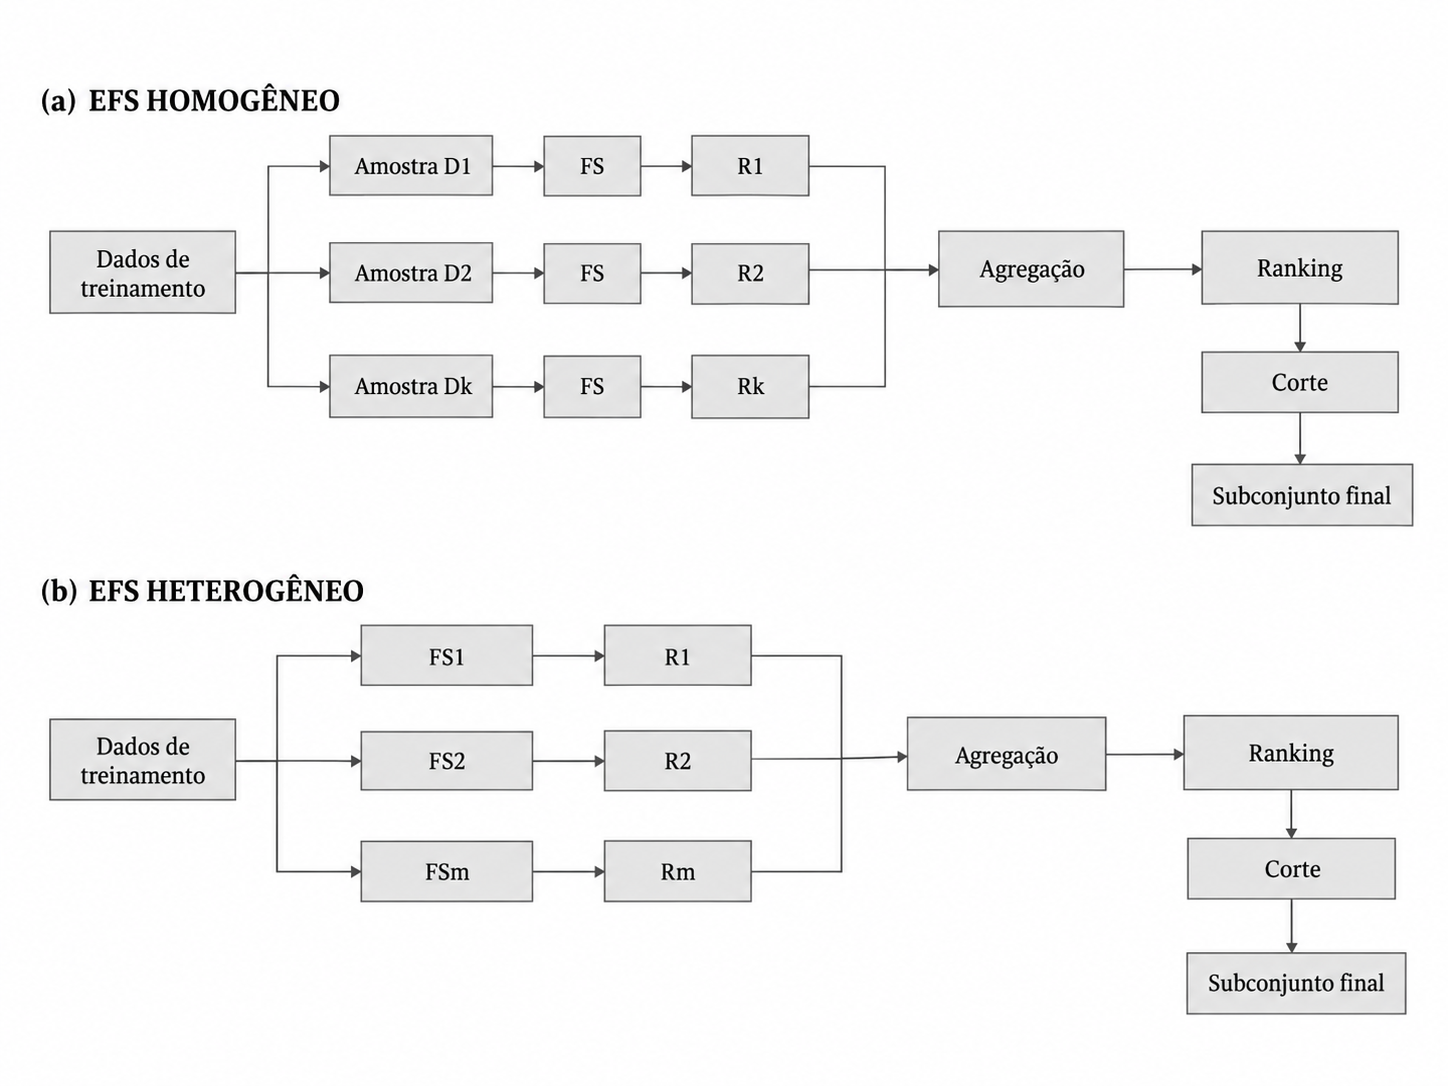
\includegraphics[width=\textwidth]
    {figuras/efs_homogeneo_heterogeneo.png}
    \caption{Estruturas gerais de \textit{Ensemble Feature Selection}
    homogêneo e heterogêneo. Elaborado pelo autor com base em
    \cite{bolon2019ensembles}.}
    \label{fig:efs_homogeneo_heterogeneo}
\end{figure}

Na Figura~\ref{fig:efs_homogeneo_heterogeneo}, $R_1,\ldots,R_k$
representam os rankings produzidos pelo mesmo seletor a partir de
diferentes amostras no EFS homogêneo, enquanto
$R_1,\ldots,R_m$ representam os rankings obtidos por diferentes
seletores no EFS heterogêneo. Em ambos os casos, os resultados
individuais são encaminhados a uma estratégia de agregação, responsável
por produzir uma representação consensual da importância dos atributos.

A forma de agregação depende do tipo de saída fornecida pelos
seletores-base. Quando os métodos produzem subconjuntos de atributos,
esses resultados podem ser combinados diretamente por estratégias de
consenso. Quando produzem rankings, diferentes métodos de agregação
podem ser utilizados para gerar um ranking global dos atributos
\cite{bolon2019ensembles}. Nesse segundo caso, torna-se necessária uma
etapa adicional de corte (\textit{thresholding}), responsável por
converter o ranking agregado em um subconjunto final de atributos.

Dessa forma, a construção de um EFS envolve três decisões fundamentais:
a geração de diversidade entre os componentes, a estratégia utilizada
para agregar os resultados individuais e o critério empregado para
determinar o subconjunto final de atributos. Essas decisões influenciam
diretamente propriedades importantes do processo de seleção, como
estabilidade, robustez e dimensionalidade do subconjunto obtido.
%%%%%%%%%%%%%%%%%%%%%
%%%%%%%%%%%%%%%%%%%
%%%%%%%%%%%%%%%%%%%
